\begin{center}
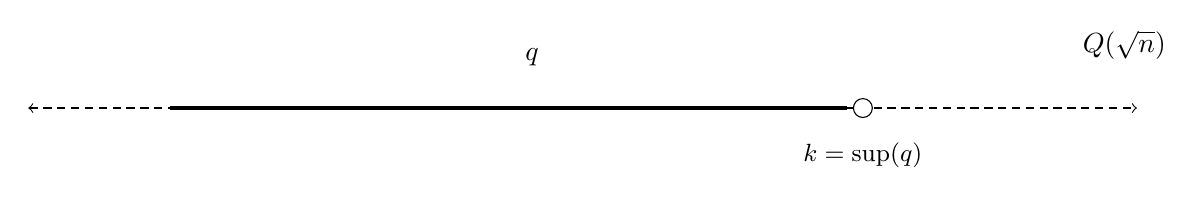
\begin{tikzpicture}[scale=4]
  \draw[<->, densely dashed] (0,2.4) -- (3.52,2.4);
  \draw[ultra thick] (0.45,2.4) -- (2.6,2.4);
  \draw[fill=white] (2.65,2.4) circle (0.03cm);
  \node[draw=none, inner sep=1.03pt] at (3.48,2.6) {$\mathbb{Q}(\sqrt{n}$)};
  \node[draw=none] at (1.6,2.56) {$q$};
  \node[draw=none, node font=\small, inner sep=1pt] at (2.65,2.25) {$k = \sup(q)$};
\end{tikzpicture}
\end{center}
